\section{Package overview}
\subsection{Description}
\prog~ is a program library for carrying out forward modelling and inversion of surface, airborne, and/or borehole magnetic data in the presence of a three dimensional Earth. The program library carries out the following functions:

\begin{enumerate}
\item Forward modelling of the magnetic field anomaly response to a 3D volume of susceptibility contrast. Data are assumed to be the \underline{anomalous} magnetic response to buried susceptible material.
\item The model is specified in the mesh of rectangular cells, each with a constant value of susceptibility. Topography is included in the mesh. The magnetic response can be calculated anywhere within the model volume, including above the topography to simulate ground or airborne surveys. There is also a capability to simulate and invert data collected beneath the surface (e.g. borehole surveys) and combinations of ground and borehole surveys.
\item Assumptions:
\begin{itemize}
\item This code assumes susceptibilities are small enough that the effects of self-demagnetization can be neglected.
\item Remanent magnetization is not directly accounted for, although anomaly projections can be included with the observations.
\end{itemize}
\item Inversion of surface, airborne, and/or borehole magnetic data to generate 3D models of susceptibility contrast:
\begin{itemize}
\item The inversion is solved as an optimization problem with the simultaneous goals of (i) minimizing an objective function on the model and (ii) generating synthetic data that match observations to within a degree of misfit consistent with the statistics of those data.
\item To counteract the inherent lack of information about the distance between source and measurement, the formulation incorporates depth or distance weighting.
\item By minimizing the model objective function, distributions of subsurface susceptibility contrast are found that are both close to a reference model and smooth in three dimensions. The degree to which either of these two goals dominates is controlled by the user by incorporating a priori geophysical or geological information into the inversion. Explicit prior information may also take the form of upper and lower bounds on the susceptibility contrast in any cell.
\item The regularization parameter (controlling relative importance of objective function and misfit terms) is determined in either of three ways, depending upon how much is known about errors in the measured data.
\end{itemize}

\item The large size of 3D inversion problems is mitigated by the use of wavelet compression. Parameters controlling the implementation of this compression are available for advanced users.
\end{enumerate}

The initial research underlying this program library was funded principally by the mineral industry consortium ``Joint and Cooperative Inversion of Geophysical and Geological Data'' (1991 - 1997) which was sponsored by NSERC (\NSERC) and the following 11 companies: BHP Minerals, CRA Exploration, Cominco Exploration, Falconbridge, Hudson Bay Exploration and Development, INCO Exploration \& Technical Services, Kennecott Exploration Company, Newmont Gold Company, Noranda Exploration, Placer Dome, and WMC.

Since then, improvements have been implemented as time and resources permit.

\subsection{\programName ~program library content}

\begin{enumerate}
\item \textbf{Executable programs}. For performing 3D forward modelling and inversion of magnetic surveys. The MAG3D library (Windows or Linux platforms) consists of four major programs: \begin{itemize}
\item \codeName{MAGFOR3D}: performs forward modelling
\item \codeName{MAGSEN3D}: calculates sensitivity and the depth weighting function
\item \codeName{MAGPRE3D}: multiplies the sensitivity file by the model to get the predicted data
\item \codeName{MAGINV3D}: performs 3D magnetic inversion.
\end{itemize}

\item \textbf{A graphical user interface}. It is available for the Windows platforms \textbf{only}. Facilities include:
\begin{itemize}
\item \codeName{GM-DATA-VIEWER}: a utility for viewing raw surface or airborne data (but not borehole data), error distributions, and for comparing observed to predicted data directly or as difference maps.
\item \codeName{MESHTOOLS3D}: a utility for displaying resulting 3D models as volume renderings. Susceptibility volumes can be sliced in any direction, or isosurface renderings can be generated.
\end{itemize}

\item \textbf{Documentation} is provided for \prog.

\item \textbf{Example data sets} are provided in ``EXAMPLES'' directory.
\end{enumerate}

\subsection{Licensing}

A \textbf{constrained educational version} of the program is available with the \href{http://www.flintbox.com/public/project/1605/}{IAG} package (please visit \href{http://gif.eos.ubc.ca}{UBC-GIF website} for details). The educational version is fully functional so that users can learn how to carry out effective and efficient 3D inversions of magnetic data. \textbf{However, RESEARCH OR COMMERCIAL USE IS NOT POSSIBLE because the educational version will NOT work with more than 200 data points or 12,000 cells in the 3D mesh}.

Licensing for an unconstrained academic version is available - see the \href{http://gif.eos.ubc.ca/software/licensing}{Licensing policy document}.

\textbf{NOTE:} All academic licenses will be \textbf{time-limited to one year}. You can re-apply after that time. This ensures that everyone is using the most recent versions of codes.

Licensing for commercial use is managed by distributors, not by the UBC-GIF research group. Details are in the \href{http://gif.eos.ubc.ca/software/licensing}{Licensing policy document}.

\subsection{Installing \prog}

There is no automatic installer currently available for the \prog. Please follow the following steps in order to use the software:

\begin{enumerate}
\item Extract all files provided from the given zip-based archive and place them all together in a new folder such as \codeName{C:\textbackslash ubcgif\textbackslash mag3d\textbackslash bin}
\item Add this directory as new path to your environment variables.
\item If you are running the software on a cluster of computers, please install the Message Pass Interface (MPI) on your computer and add it to your path in addition.
\item Make sure to create a separate directory for each new inversion, where all the associated files will be stored. Do not store anything in the ``bin'' directory other than executable applications and Graphical User Interface applications (GUIs).
\end{enumerate}

\subsection{\prog: Highlights of changes from version \preV}

The principal upgrades, described below, allow the new code to take advantage of current multi-core computers and also provide greater flexibility to incorporate the geological information.

Improvements since version \preV~:

\begin{enumerate}
\item A new projected gradient algorithm is used to implement constraints.
\item Fully parallelized computational capability (for both sensitivity matrix calculations and inversion calculations).
\item An alternative version of the software compatible with Message Pass Interface (MPI) is available.
\item A facility to have active and inactive (i.e. fixed) cells is implemented
\item Additional flexibility is added when using the reference model in the model objective function
\end{enumerate}

\subsection{Notes on computation speed}
\begin{itemize}
\item The execution time using \programName~\preV~ and \version~ are compared in Figure \ref{fig:Speed} for a moderately complicated problem. This was a synthetic example involving 3,600 data points and 131,072 cells in the model, and moderate topography.
\item The version \version~code is significantly faster in all cases due to parallelization of sensitivity matrix computation and inversion calculations.
\item Speed is dependent upon the computer. It is strongly recommended to use multicore processors for running the \codeName{magsen3d} and \codeName{mag3d}. The calculation of the sensitivity matrix (\textbf{G}) is directly proportional to the number of data. The parallelization of \textbf{G} calculation splits the calculation of $n$ rows between $p$ processors. By default, all available processors are used. There is a feature to limit $p$ to user-defined number of processors.
\item In the parallelized inversion calculation, $\mathbf{G}^T \mathbf{G}$ is multiplied by a vector, therefore each parallel process uses only a submatrix of $\mathbf{G}$ and then the calculations are summed. Since there is a lot of communication between the CPUs, the speedup may be less than directly proportional to the number of processors, however when running the same inversion under MPI environment on multiple computers the advantage is that a single computer does not have to store the entire sensitivity matrix.
\item Using a single thread for running the parallelized version resulted in sensitivity matrix calculation slowdown exactly proportional to the reduction in number of threads, while the slowdown in inversion calculation was insignificant (21.7 seconds with 1 thread vs 18.18 seconds with 12 threads).
\item The implementation of the ``projected gradient'' algorithm in version \version~ versus the ``logarithmic barrier'' algorithm in version ~\preV results in faster convergence (11 iterations versus 33 iterations, respectively) with almost identical result (the recovered susceptibility models have been compared and their mismatch is under 0.4\%).
\item The complexity of the problem also affects computation times. More complex problems include topography, complicated distributions of susceptibility, weighting functions, reference models, bounds, etc.
\item These results are presented for illustration only. The time to compute any given problem is strongly dependent upon the number of data points, the size of the mesh, and how all the parameters for the inversion are set, including data, constraints, regularization, wavelet compression, etc.
\end{itemize}

\begin{figure}
\center
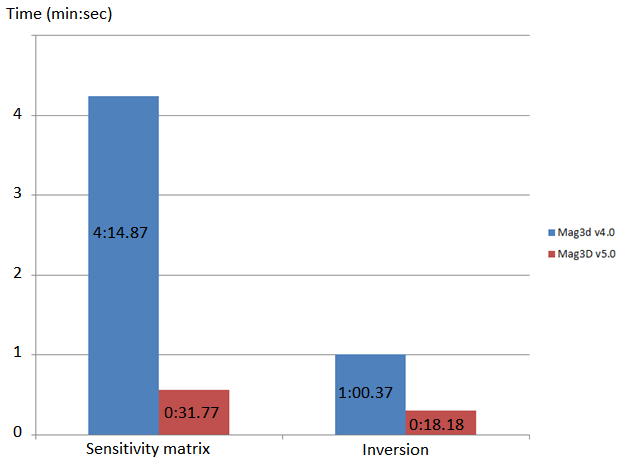
\includegraphics[width=0.7\columnwidth]{Speed}
\caption{CPU time on 3.20 GHz 6 core i7 Intel processor with 16 Gb of RAM installed. Twelve parallel OpenMP threads were used for the calculations in version \version.}
\label{fig:Speed}
\end{figure}
